% Document class and parameters %
\documentclass[10pt,a4paper]{article}

% Document packages %
\usepackage{graphicx}
\usepackage{biblatex}
\usepackage{parskip}
\usepackage{listings}
\usepackage{caption}
\usepackage{subcaption}
\usepackage{amsmath}
\usepackage[most]{tcolorbox}


\graphicspath{{./Images/}}
\setlength{\parskip}{1em}

% Document Body %
\begin{document}
\begin{titlepage}
	\centering
	{\scshape\LARGE Imperial College London \par}
	\vspace{1cm}
	{\scshape\Large Mathematics: Year 2\par}
	\vspace{1.5cm}
	{\huge\bfseries Events, Probability and Sets\par}
	\vspace{2cm}
	{\Large\ Xin Wang }
	\vfill
	{\large \today\par}
\end{titlepage}

\begin{abstract}
Engineering is a profession founded upon experimentation, the data it produces, and how it is
extracted and analysed. 

\textbf{Probability} is the mathematical science of dealing with uncertainty - it provides engineers with the
rules for analyzing and understanding ignorance about uncertain situations.

\textbf{Statistics} is the science of reasoning about data in the presence of uncertainty that can
arise for numerous reason in the real world such as noise. In the real world, data collected is composed of signal
and noise that needs to be spilt and analysed.
\end{abstract}

\tableofcontents
\pagebreak

%%%%%%%%%%%%%%%%%%%%%%%%%%%%%%%%%%%%%%%%%%%%%%%%%%%%%%%%%%%%%%%%%%%%%%%%%%%%%%%%%%%%%%%%%%%%%%%%%%%%%%%%%%
\section{Sets}

\begin{tcolorbox}[breakable,colback=white]
\textbf{Set}: A collection of unordered, distinct objects (\textbf{elements}).
\\
\\
\textbf{Cardinality}: A measure of the number of elements of a set.
\\
\\
\textbf{Singleton}: A set with a single element.
\end{tcolorbox}

Notations:
\begin{itemize}
    \item If an element denoted as $\omega$ is part of set $A$, formally defined as "$\omega$ belongs to $A$":
    $$
        \omega \in A
    $$
    
    \item Contents of sets are enclosed in curly braces ${\dots}$
    $$
        A = \left\{\omega, 1, A\right\}
    $$
\end{itemize}

A set can contain any mixture of different objects e.g. a set containing integer, letter and other
sets. Practically, the type of elements a set can have is usually restricted to a
\textbf{collection} of possible values. This collection \textbf{is a set itself} called the
\textbf{universal set} ($\Omega$).


\begin{tcolorbox}[breakable,colback=white]
\textbf{Empty set} ($\phi$ = \{\}): A unique set that contains no elements.
\end{tcolorbox}

Set relation notation:
\begin{itemize}
    \item $\subseteq$: $A$ is a \textbf{subset} of $B$ - all elements of $A$ are members of $B$ with the
    possibility that set $A$ is equal (contain the same elements) as set $B$ i.e. $A\subseteq B$
    \item $\subset$: $A$ is a \textbf{proper subset} of $B$ - all elements of $A$ are members of $B$
    and set $A$ must be smaller than set $B$
    \item $=$: $A$ and $B$ have the identical elements i.e. $A\subseteq B$ and $B \subseteq A$ thus $A=B$ 
\end{itemize}

%%%%%%%%%%%%%%%%%%%%%%%%%%%%%%%%%%%%%%%%%%%%%%%%%%%%%%%%%%%%%%%%%%%%%%%%%%%%%%%%%%%%%%%%%%%%%%%%%%%%%%%%%%
\section{Sets and Set operations}
%%%%%%%%%%%%%%%%%%%%%%%%%%%%%%%%%%%%%%%%%%%%%%%%%%%%%%%%%%%%%%%%%%%%%%%%%%%%%%%%%%%%%%%%%%%%%%%%%%%%%%%%%%
\subsubsection{Union}

\begin{tcolorbox}[breakable,colback=white]
\textbf{Union} $(A \cup B)$: The set containing all elements in $A$ alone, all elements in
$B$ alone \textbf{and} all elements shared by both $A$ and $B$.
$$
    A \cup B = \left\{\omega \in \Omega\; : \; \omega \in A \text{ \textbf{or} }\omega \in B\right\} 
$$
\end{tcolorbox}

Properties of union:
\begin{itemize}
    \item Identity law: $A\cup \phi = A$
    \item Idempotent law: $A \cup A = A$
    \item Domination law: $A \cup \Omega = \Omega$
    \item Commutative law: $A\cup B = B \cup A$
\end{itemize}

%%%%%%%%%%%%%%%%%%%%%%%%%%%%%%%%%%%%%%%%%%%%%%%%%%%%%%%%%%%%%%%%%%%%%%%%%%%%%%%%%%%%%%%%%%%%%%%%%%%%%%%%%%
\subsection{Intersection}

\begin{tcolorbox}[breakable,colback=white]
\textbf{Intersection} $(A \cap B)$: The set containing all elements that
belong to both $A$ and $B$.
$$
    A \cap B = \left\{\omega \in \Omega\; : \; \omega \in A \text{ \textbf{and} }\omega \in B\right\}
$$
\end{tcolorbox}

Properties of union:
\begin{itemize}
    \item Identity law: $A\cap \phi = \phi$
    \item Idempotent law: $A \cap A = A$
    \item Domination law: $A \cap \Omega = A$
    \item Commutative law: $A\cap B = B \cap A$
\end{itemize}

%%%%%%%%%%%%%%%%%%%%%%%%%%%%%%%%%%%%%%%%%%%%%%%%%%%%%%%%%%%%%%%%%%%%%%%%%%%%%%%%%%%%%%%%%%%%%%%%%%%%%%%%%%
\subsection{Combination of union and intersection}

The combination of Union and Intersection results in the Distributive Law:
\begin{itemize}
    \item $A \cup(B\cap C)=(A\cup B)\cap (A\cup C)$
    \item $A \cap (B \cup C) = (A\cap B) \cup (A\cap C)$ 
\end{itemize}

%%%%%%%%%%%%%%%%%%%%%%%%%%%%%%%%%%%%%%%%%%%%%%%%%%%%%%%%%%%%%%%%%%%%%%%%%%%%%%%%%%%%%%%%%%%%%%%%%%%%%%%%%%
\subsection{Disjoint and partition}

\textbf{Disjoint}: If sets $A$ and $B$ share no elements: 
$$
    A \cap B = \phi
$$
Common result of disjoint: $A \cap \overline{A} = \phi$

\textbf{Partition of $\Omega$}: If a collection of sets $A_1,A_2,\dots,A_n$ are disjoint and the
union of the sets equals the \textbf{universal set}.
$$
    \bigcup_{i=1}^n A_i = \Omega
$$
Common result of disjoint: $A \cup \overline{A} = \Omega$

%%%%%%%%%%%%%%%%%%%%%%%%%%%%%%%%%%%%%%%%%%%%%%%%%%%%%%%%%%%%%%%%%%%%%%%%%%%%%%%%%%%%%%%%%%%%%%%%%%%%%%%%%%
\subsection{Complements and Differences}

\begin{tcolorbox}[breakable,colback=white]
\textbf{Complements} (of a set): The set that contains all elements of $\Omega$ that do not belong
to $A$ - not $A$.
$$
    \overline{A}
$$
\end{tcolorbox}

Properties of union:
\begin{itemize}
    \item $\overline{(\overline{A})}=A$
    \item $\overline{\phi}=\Omega$
    \item $A \cup \overline{A}=\Omega$
    \item $A \cap \overline{A}=\phi$
\end{itemize}

\begin{tcolorbox}[breakable,colback=white]
\textbf{Difference} (of sets $A$ and $B$): The set that contains elements of set $A$ that do not
belong to set $B$.
$$
    A/B = \left\{\omega\in \Omega\; :\; \omega\in A \text{ and }\omega \notin B\right\}
$$
\end{tcolorbox}

The two sets $A$ and $B$ are disjoint sets if $A/B=A$. The difference of two sets can be interpreted
as:
$$
    A/B = A \cap \overline{B}
$$
and
$$
    \overline{A} = \frac{\Omega}{A}
$$

%%%%%%%%%%%%%%%%%%%%%%%%%%%%%%%%%%%%%%%%%%%%%%%%%%%%%%%%%%%%%%%%%%%%%%%%%%%%%%%%%%%%%%%%%%%%%%%%%%%%%%%%%%
\subsection{De Morgan's laws}

De Morgan's laws allows the combination of complements, unions and intersections.
\begin{align*}
    \overline{(A \cup B)} = \overline{A} \cap \overline{B} \\
    \overline{(A\cap B)} = \overline{A} \cup \overline{B}
\end{align*}

%%%%%%%%%%%%%%%%%%%%%%%%%%%%%%%%%%%%%%%%%%%%%%%%%%%%%%%%%%%%%%%%%%%%%%%%%%%%%%%%%%%%%%%%%%%%%%%%%%%%%%%%%%
\section{Sample spaces and Events}

Consider a \textbf{random experiment} where the outcome is unknown and all the possible
outcomes can be described by the \textbf{sample space} i.e. a non-empty set denoted $S$.

\textbf{Example 1}: Find the sample space of a toss of a coin.
$$
    S = \left\{H,\:T\right\}
$$

Often, establishing whether a sample space is \textbf{discrete} or \textbf{continuous} is important and
affects the techniques used to analyse and find the answer.

\textbf{Example 2}: Find the sample space of the thickness of a molded plastic container.
\begin{itemize}
    \item Discrete:
    $$
        S = \left\{low,\: medium,\: high\right\}
    $$

    \item Continuous:
    $$
        S =\left\{x: 20 < x < 30\right\}
    $$
\end{itemize}

\begin{tcolorbox}[breakable,colback=white]
\textbf{Events}: Subsets of the sample space i.e. possible outcomes.
\end{tcolorbox}

\textbf{Example 3}: List the possible events that could occur from a coin toss given the sample space:
\begin{align*}
    S = \left\{H, T\right\}
\end{align*}

Possible events are:
\begin{align*}
    E = \left\{H\right\} \; \text{and}\; E=\left\{T\right\}
\end{align*}
In the context of random events, there are several special events:
\begin{itemize}
    \item \textbf{Null event}: An empty set - $\phi$ i.e. never occurs.
    \item \textbf{Elementary event} (of $S$): An event that is a \textbf{singleton subset} of $S$.
    \item \textbf{Universal event}: The sample space $S$ that consists of the union of all elementary events.
\end{itemize}

%%%%%%%%%%%%%%%%%%%%%%%%%%%%%%%%%%%%%%%%%%%%%%%%%%%%%%%%%%%%%%%%%%%%%%%%%%%%%%%%%%%%%%%%%%%%%%%%%%%%%%%%%%
\section{Probability axioms}

\textit{Axioms - A statement/proposition that is regarded as being already well established.}

To be able to understand the uncertainty of an event, a set function $P$ called the \textbf{probability
function} or \textbf{probability measure} is defined. $P$ takes a set as argument and returns
a value.

In order for a set function to be the probability for any event that is a subset of the sample
space, defined mathematically as $E \subseteq S$, it has to satisfy three conditions:
\begin{enumerate}
    \item $0 \leq P(E) \leq 1$: Where $1$ as occurring and $0$ not occurring.
    \item $P(S) = 1$: The sample space contains all the possible events thus will occur.
    \item If two events are independent and does not overlap $E\cap F = \phi$, then $P(E\cup
    F)=P(E)+P(F)$: The probability of either event occurring are not related thus can be the sum of
    probability of each specified event occurring.
\end{enumerate}

\begin{tcolorbox}[breakable,colback=white]
Given three disjoint subsets $E_1,E_2,\dots,E_i \in S$, the probability of either event occurring is the
\textbf{sum of probability of each specified event occurring}:
$$
    P\left(\bigcup_i E_i\right) = \sum_i P(E_i)
$$
\end{tcolorbox}

Understanding the three axioms allows several important relationships to be established:
\begin{enumerate}
    \item Probability of an event occurring and the probability of the event not
    occurring must add up to 1:
    \begin{align*}
        P(E)+P(\overline{E})=P(S)=1 \\
        P(E) = 1-P(\overline{E})
    \end{align*}
    Able to compute $P(\overline{E})$ from knowing $P(E)$.

    \item Boole's relationship: Union of events $E$ and $F$:
    \begin{align*}
        E \cup F = E\cup \left(\overline{E}\cap F\right) \Rightarrow P(E\cup F) = P(E)+P(\overline{E}\cap F)
    \end{align*}
    and
    \begin{align*}
        F=(E\cap F) \cup (\overline{E}\cap F) \Rightarrow P(F)=P(E\cap F)+P(\overline{E}\cap F)
    \end{align*}
    combine to form Boole's relationship:
    \begin{align*}
        P(E\cup F)=P(E)+P(F)-P(E\cap F)
    \end{align*}
    
    \item Probability of union $E$ and $F$ is \textbf{less than or equal to} sum of individual
    probabilities of event $E$ and $F$:
    
    If two events are not disjoint $P(E \cap F)\geq 0$:
    \begin{align*}
        P(E\cup F) \leq P(E) +P(F)
    \end{align*}

    \item The highest possibility between two events will always be less than probability of either
    event occurring which is less than probability sum of two events occurring.
    \begin{align*}
        max[P(E),P(F)] \leq P(E\cup F) \leq P(E)+P(F)
    \end{align*}

    \item Probability of either events $E$ and $F$ not occurring is less than the probability of
    both events occurring which is less than the lowest probability between two events.
    \begin{align*}
        P(E)+P(F)-1\leq P(E\cap F) \leq min[P(E),P(F)]
    \end{align*}

    \item Poincare's formula:
    $$
        P(A\cup B \cup C)=P(A)+P(B)+P(C)-P(C\cap A)-P(C\cap B)-P(A\cap B)+P(C\cap A\cap B)
    $$
\end{enumerate}

\textbf{Example 1}: Consider events $A$ and $B$ and the given probabilities:
\begin{itemize}
    \item $P(A)=P(B)=0.90$
    \item $P(A\cap B)=0.85$
\end{itemize}

Find $P(A \cup B)$:
\begin{align*}
    P(A \cup B) &= P(A)+P(B) - P(A\cap B) \\
    &= 2 \times 0.9 - 0.85 \\
    &= 0.95
\end{align*}

Find $P(\overline{A}\cap B)$:
\begin{align*}
    P(\overline{A}\cap B) &= P(B)-P(A\cap B)\\
    &= 0.05
\end{align*}

%%%%%%%%%%%%%%%%%%%%%%%%%%%%%%%%%%%%%%%%%%%%%%%%%%%%%%%%%%%%%%%%%%%%%%%%%%%%%%%%%%%%%%%%%%%%%%%%%%%%%%%%%%
\section{Probability computation}

\begin{tcolorbox}[breakable,colback=white]
\textbf{Probability}: In a sample space $S$ with $n$ number of \textbf{equally possible}
events, the probability of a event defined as $E \subseteq S$:
\begin{align*}
    P(E) = \frac{\text{events in }E}{n}
\end{align*}
\end{tcolorbox}

\textbf{Example 1}: Given a 6-faced die with sample space $S = \left\{1,2,3,4,5,6\right\}$, find the
probability of rolling an even number.
\begin{enumerate}
    \item Find $n$:
    $$
        P(S)=\frac{1}{6}
    $$

    \item Probability of an even number:
    $$
        P(E) = P(2 \cup 4 \cup 6) = \frac{1}{2}
    $$
\end{enumerate}

\textbf{Addition rule of probability}: 
\begin{align*}
    P(A\cup B) = P(A) + P(B)-P(A\cap B)
\end{align*}

\textbf{Example 2}: Consider drawing a random card from a deck of cards:
\begin{itemize}
    \item $A$ defined as the event of drawing a heart with probability $P(A)=\frac{13}{52}=\frac{1}{4}$
    \item $B$ defined as the even of drawing cards $\left\{J, Q, K\right\}$ with probability $P(B)=\frac{12}{52}=\frac{3}{13}$
    \item Since $A$ and $B$ are not disjoint as some face cards are also hearts, $P(A\cap B)=\frac{3}{52}$
\end{itemize}

The probability of $A$ or $B$ is defined as:
\begin{align*}
    P(A \cup B) &= P(A) + P(B) - P(A\cap B) \\
    &= \frac{1}{4} + \frac{3}{13} + - \frac{3}{52} \\
    &= \frac{11}{26} 
\end{align*}

%%%%%%%%%%%%%%%%%%%%%%%%%%%%%%%%%%%%%%%%%%%%%%%%%%%%%%%%%%%%%%%%%%%%%%%%%%%%%%%%%%%%%%%%%%%%%%%%%%%%%%%%%%
\section{Conditional Probability}

\textbf{Conditional probability}: The concept of describing the probability of an event \textbf{given that
another event has already occurred}. This concept is important as usually events are influenced by other events.

The common notation defined as:
\begin{center}
    \textit{"the probability that event $A$ occurs given that $B$ has already occurred"}
\end{center} 
$$
    P(A|B)
$$

\begin{tcolorbox}[breakable,colback=white]
For events $A$ and $B$ where $P(B)>0$, the \textbf{conditional probability} $P(A|B)$ is defined as:
$$
    P(A|B) = \frac{P(A\cap B)}{P(B)}
$$
\end{tcolorbox}

Due to the conditioning event, the conditional probability considers a reduced subset of the sample
space.
\begin{itemize}
    \item If $B\subseteq A$:
    \begin{align*}
        P(A|B) = \frac{P(A\cap B)}{P(B)} = \frac{P(B)}{P(B)} = 1 \geq P(A)
    \end{align*}

    If $B$ is a subset of $A$, the probability of an event in $B$ as well in $A$ [$P(A\cap B)$] occurring is
    basically the probability of $B$ [$P(B)$]. This means that when finding the probability of $A$
    occurring given that $B$ has occurred already and $B$ is a subset of $A$, the event $A$ has
    already occurred.

    \item If $A \cap B = \phi$
    \begin{align*}
        P(A|B) = \frac{P(A\cap B)}{P(B)} = \frac{0}{P(B)} = 0 \leq P(A)
    \end{align*} 

    If there are no common events in $A$ and $B$, set $B$ does not affect the probabilities of
    events in $A$ occurring. 
\end{itemize}

\textbf{Multiplication law of probability}: 
$$
    P(A \cap B) = P(A)P(B|A)
$$
it follows that:
$$
    P(A|B)P(B) = P(A \cap B)=P(A)P(B|A)
$$

The result shows the relationship between conditional probabilities and unconditional probabilities.

\textbf{Example 1}: When throwing a dice, let $A = \left\{\text{even number}\right\}$ and
$B=\left\{\text{score}\geq 3\right\}$:
\begin{itemize}
    \item $P(A)=\frac{1}{2}$
    \item $P(B)=\frac{2}{3}$
    \item $P(A\cap B)=\frac{1}{3}$
\end{itemize}

Then the difference between $P(A|B)$ and $P(B|A)$ are as follows:
\begin{itemize}
    \item $P(A|B)$:
    \begin{align*}
        P(A|B) &= \frac{P(A\cap B)}{P(B)} \\
        &= \frac{\frac{1}{3}}{\frac{2}{3}} \\
        &= \frac{1}{2}
    \end{align*}

    \item $P(B|A)$:
    \begin{align*}
        P(B|A) &= \frac{P(B\cap A)}{P(A)} \\
        &= \frac{\frac{1}{3}}{\frac{1}{2}} \\
        &=\frac{2}{3}
    \end{align*}
\end{itemize}

%%%%%%%%%%%%%%%%%%%%%%%%%%%%%%%%%%%%%%%%%%%%%%%%%%%%%%%%%%%%%%%%%%%%%%%%%%%%%%%%%%%%%%%%%%%%%%%%%%%%%%%%%%
\subsection{Independence}

Given the concept of conditional probability, the concept of \textbf{independence} can be defined.

\begin{tcolorbox}[breakable,colback=white]
\textbf{Independence}: The occurrence of one event does not change the probability of the occurrence
of another event.
\\
\\
Events $A$ and $B$ are said to be independent if:
$$
    P(A|B) = P(A)
$$
\end{tcolorbox}

For independent events, the multiplication rule results:
$$
    P(A\cap B) = P(A|B)P(B) = P(A)P(B)
$$

This results shows that independent events having multiplicative probabilities is a critical concept
that leads to \textbf{mutual independence}:
$$
    P(A_1 \cap A_2 \cap \dots \cap A_n) = P(A_1)P(A_2)\dots P(A_n)
$$

\textbf{Example 1}: Given a dice with two events $A=\left\{1,2,3\right\}$ and
$B=\left\{2,4\right\}$, proof the two events are independent.
\begin{itemize}
    \item $P(A)=\frac{1}{2}$
    \item $P(B)=\frac{1}{3}$
    \item $P(A\cap B)=\frac{1}{6}$
\end{itemize}

Process:
\begin{enumerate}
    \item Find $P(A|B)$:
    \begin{align*}
        P(A|B) &= \frac{P(A\cap B)}{P(B)} \\
        &= \frac{\frac{1}{6}}{\frac{1}{3}} \\
        &= \frac{1}{2}\\
        &= P(A)
    \end{align*}

    \item Find $P(B|A)$:
    \begin{align*}
        P(B|A) &= \frac{P(B\cap A)}{P(A)} \\
        &= \frac{\frac{1}{6}}{\frac{1}{2}} \\
        &= \frac{1}{3}\\
        &= P(B)
    \end{align*}

    \item Conclude $P(A|B)=P(A)$ and $P(B|A)=P(B)$ thus $A$ and $B$ are independent.
\end{enumerate}

%%%%%%%%%%%%%%%%%%%%%%%%%%%%%%%%%%%%%%%%%%%%%%%%%%%%%%%%%%%%%%%%%%%%%%%%%%%%%%%%%%%%%%%%%%%%%%%%%%%%%%%%%%
\section{Probability tables}

Information regarding the probability of pairs of events and their complements can be conveniently
represented as a \textbf{probability table}.

\begin{figure} [h!]
    \centering
    \includegraphics[scale=0.5]{prob table.JPG}
\end{figure}

The table represents disjoint unions i.e. $P(A)+P(\overline{A})=1$ or $P(A)=P(A\cap B)+P(A\cap
\overline{B})$.

\textbf{Example 1}: Given 100 girders, faults of type $A$ and $B$ are checked. 
\begin{itemize}
    \item 2 have both types of faults - $A\cap B$ 
    \item 6 have type $A$ fault - $A\cap \overline{B}$
    \item 4 have type $B$ fault - $\overline{A}\cap B$
\end{itemize}

\begin{figure} [h!]
    \centering
    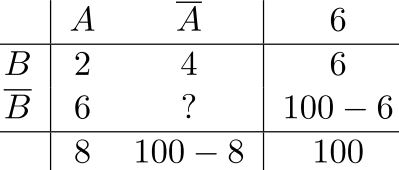
\includegraphics[scale=0.5]{Prob table 2.JPG}
\end{figure}

Conditional probability calculations are straight forward:
\begin{itemize}
    \item $P(A|B)=\frac{1}{3}$
    \item $P(B|A)=\frac{2}{8}\frac{1}{4}$
    \item Probability of one fault: 
    \begin{align*}
        P((A\cap \overline{B})\cup (\overline{A}\cap B)) &= P(A\cap \overline{B}) + P(\overline{A}\cap B) \\
        &= \frac{6}{100}+\frac{4}{100} \\
        &= \frac{1}{10}
    \end{align*}
\end{itemize}

%%%%%%%%%%%%%%%%%%%%%%%%%%%%%%%%%%%%%%%%%%%%%%%%%%%%%%%%%%%%%%%%%%%%%%%%%%%%%%%%%%%%%%%%%%%%%%%%%%%%%%%%%%
\section{Total probability}

Previous chapters mentioned that a collection of disjoint sets $A_1,A_2,\dots,A_n$ forms a
\textbf{partition} of $S$ if $A_i \cap A_j = \phi$ thus:
$$
    S = \bigcup_{i=1}^k A_i
$$

Therefore for any event $B$:
$$
    B = (B\cap A_1)\cup \dots \cup (B\cap A_k) \Rightarrow P(B)=P(B\cap A_1)+\dots+P(B\cap A_k)
$$

Each event can be written in terms of the multiplication law to yield:
$$
    P(B)=P(B|A_1)P(A_1)+\dots+P(B|A_k)P(A_k) = \sum_{i=1}^k P(B|A_i)P(A_i)
$$

\begin{figure} [h!]
    \centering
    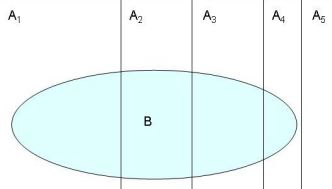
\includegraphics[scale=0.7]{partition.JPG}
\end{figure}

\begin{tcolorbox}[breakable,colback=white]
For events $A_1,A_2,\dots,A_k$ such that $A_i\cap A_j=\phi$:
\begin{itemize}
    \item For all $i$ and $j$
    \item $i \neq j$
    \item $\bigcup_{i=1}^k A_i = S$
\end{itemize} 
the theorem of total probability states:
$$
    P(B)=\sum_{i=1}^k P(B|A_i)P(A_i)
$$
\end{tcolorbox}

\textbf{Example 1}: Consider a factory with 3 machines $X$, $Y$ and $Z$ that is used to produce a
specific component and each that a different defect probability:
\begin{itemize}
    \item $X$: Produces $50\%$ of components with $3\%$ defective.
    \item $Y$: Produces $30\%$ of components with $4\%$ defective. 
    \item $Z$: Produces $20\%$ of components with $5\%$ defective. 
\end{itemize} 
Compute the probability that a randomly selected item is a defect.

Process:
\begin{enumerate}
    \item $D$ denotes the event concerned:
    $$
        D = (D \cap X) \cup (D\cap Y) \cup (D\cap Z)
    $$

    \item Apply the law of total probability:
    \begin{align*}
        P(D) &= P(D|X)P(X)+P(D|Y)P(Y)+P(D|Z)P(Z) \\
        &= 0.03(0.5) + 0.04(0.3) + 0.05(0.2) \\
        &= 0.037
    \end{align*}
\end{enumerate}

%%%%%%%%%%%%%%%%%%%%%%%%%%%%%%%%%%%%%%%%%%%%%%%%%%%%%%%%%%%%%%%%%%%%%%%%%%%%%%%%%%%%%%%%%%%%%%%%%%%%%%%%%%
\section{Bayes Theorem}

Bayes Theorem is also commonly known as the rule for switching conditional probabilities.

For events $A_1,\dots,A_n$ that form a partition of $S$ and any other event $B$, the multiplication rule
for conditional probability states:
$$
    P(A_k \cap B) = P(A_k)P(B|A_k)
$$
Therefore:
$$
    P(A_k|B) = \frac{P(A_k\cap B)}{P(B)} = \frac{P(A_k)P(B|A_k)}{P(B)}
$$

The term in the denominator can be expressed as terms of conditional probabilities via the theorem
of total probability.

\begin{tcolorbox}[breakable,colback=white]
\textbf{Bayes Theorem}:
\\
For events $A_1,\dots,A_n$ that form a partition of $S$ and any other event $B$:
$$
    P(A_k|B) = \frac{P(A_k)P(B|A_k)}{P(A_1)P(B|A_1)+\dots+P(A_n)P(B|A_n)}
$$
\end{tcolorbox}

Bayes Theorem provides the ability to determine the probability that a particular event $A$
\textbf{occurred} given that event $B$ has \textbf{already occurred}.

\textbf{Example 1}: Building on the previous example, suppose a defective component is found among the output of a factory, find the
probability that it came from each of the machines $X$, $Y$ and $Z$. $P(D)$ is already calculated to
be $0.037$.
\begin{itemize}
    \item Find $P(X|D)$:
    \begin{align*}
        P(X|D) = \frac{P(D|X)P(X)}{P(D)} = \frac{0.03(0.5)}{0.037} = 0.4054
    \end{align*}

    \item Find $P(Y|D)$:
    \begin{align*}
        P(Y|D) = \frac{P(D|Y)P(Y)}{P(D)} = \frac{0.04(0.3)}{0.037} = 0.3243
    \end{align*}

    \item Find $P(Z|D)$:
    \begin{align*}
        P(Z|D) = \frac{P(D|Z)P(Z)}{P(D)} = \frac{0.05(0.2)}{0.037} = 0.2703
    \end{align*}
\end{itemize}

%%%%%%%%%%%%%%%%%%%%%%%%%%%%%%%%%%%%%%%%%%%%%%%%%%%%%%%%%%%%%%%%%%%%%%%%%%%%%%%%%%%%%%%%%%%%%%%%%%%%%%%%%%
\end{document}